\documentclass{article}
\usepackage{amsfonts,amsthm,amsmath,amssymb,mathtools}
\usepackage{mathrsfs}
\usepackage{enumitem}
\usepackage{tikz-cd}

% Chapter
\newcounter{chapter}
\setcounter{chapter}{2}

% Section
\setcounter{section}{2}

\newtheorem{thm}{Theorem}
\newenvironment{theorem}[1]{
	\renewcommand{\thethm}{#1}
	\begin{thm}
		}{\end{thm}}

\newtheorem{lma}{Lemma}
\newenvironment{lemma}[1]{
	\renewcommand{\thelma}{#1}
	\begin{lma}
		}{\end{lma}}

\theoremstyle{definition}
\newtheorem{ex}{}[section]
\newenvironment{exercise}[1]{
  \renewcommand{\theex}{\arabic{section}.\arabic{ex}}
	\begin{ex}
		}{\end{ex}}

\title{Exercises {\Roman{chapter}}.{\arabic{section}}}
\author{Connor Mooneyhan}
\date{July 2, 2024}

\begin{document}

\maketitle

\begin{ex}
	One can associate an $n \times n$ matrix $M_\sigma$ with a permutation $\sigma \in S_n$, by letting the entry at $(i, (i)\sigma)$ be 1 and letting all other entries be 0.
	For example, the matrix corresponding to the permutation \begin{equation*}
		\sigma = \begin{pmatrix*}
			1 & 2 & 3 \\
			3 & 1 & 2
		\end{pmatrix*} \in S_3
	\end{equation*}
	would be \begin{equation*}
		M_\sigma = \begin{pmatrix*}
			0 & 0 & 1 \\
			1 & 0 & 0 \\
			0 & 1 & 0
		\end{pmatrix*}.
	\end{equation*}
	Prove that, with this notation, \begin{equation*}
		M_{\sigma r} = M_\sigma M_r
	\end{equation*}
	for all $\sigma, r \in S_n$, where the product on the right is the ordinary product of matrices.
\end{ex}
\begin{proof}
	First, observe that each $M_\sigma$ has exactly one nonzero element in each row and each column.
	For rows, this is because $\sigma$ is a function, so $(i)\sigma$ has exactly one value.
	For columns, there must be at least one element in each column because $\sigma$ is surjective, and since $\sigma$ is injective, there cannot by two or more entries since that would imply $(i_1)\sigma = (i_2)\sigma$ for some $i_1 \neq i_2$.

	We clarify that $\sigma r$ applies $\sigma$ \textit{before} $r$ and $M_\sigma M_r$ applies $M_\sigma$ \textit{after} $M_r$.
	We denote the entry in row $j$, column $k$ of $M_\sigma$ by $a_{j,k}$ and the same in $M_r$ by $b_{j, k}$.
	By definition, the entry in row $j$, column $k$ in $M_\sigma M_r$ is \begin{equation*}
		\sum_{m = 1}^n a_{j, m}b_{m, k},
	\end{equation*}
	which has nonzero terms when $(j)\sigma = m$ and $(m)r = k$.
	Thus the only nonzero (and thus, valued 1) entries are those where $((j)\sigma)r = k$, which is exactly the definition of the nonzero entries of $M_{\sigma r}$.
\end{proof}

\begin{ex}
	Prove that if $d \leq n$, then $S_n$ contains elements of order $d$.
\end{ex}
\begin{proof}
	We proceed by induction over $n$.
	Clearly the conclusion holds for $S_1$ since the identity has order $1$.
	Thus, assume that, for some $n$, the theorem holds for $S_{n - 1}$.
	Let $\sigma_d \in S_{n-1}$ be an element of order $d$ for each $d \leq n - 1$.
	Then the permutation $f_d \in S_n$ defined by \begin{equation*}
		f_d(x) = \begin{cases}
			\sigma_d(x) & x < n \\
			x           & x = n
		\end{cases}
	\end{equation*}
	has order $d$ since if $x < n$, then $f_d^d(x) = \sigma_d^d(x) = x$ (and for some such $x$, this holds for no value less than $d$) by definition of $\sigma_d$, and if $x = n$, then obviously $f_d^d(x) = x$.

	If $d = n$, then we show that the ``rightward shift'' permutation is of order $d$.
	Indeed, define $f_n$ by \begin{equation*}
		\begin{pmatrix*}
			1 & 2 & \cdots & n \\
			2 & 3 & \cdots & 1
		\end{pmatrix*},
	\end{equation*} and we see that $f_n^n(x) = x$ for each $x$, but this holds for no other value less than $n$, so $|f_n| = n$.
\end{proof}

\begin{ex}
	For every positive integer $n$ find an element of order $n$ in $S_{\mathbb{N}}$.
\end{ex}
\begin{proof}
	Define $\sigma_n \in S_{\mathbb{N}}$ by \begin{equation*}
		\sigma_n(x) = \begin{cases}
			(x + 1) \bmod n & 0 \leq x < n                 \\
			x               & x < 0\ \mathrm{or}\ x \geq n
		\end{cases}
	\end{equation*}
	That this has order $n$ is a feature of elementary modular arithmetic.
\end{proof}

\begin{ex}
	Define a homomorphism $D_8 \to S_4$ by labelling vertices of a square, as we did for a triangle in \S 2.2.
	List the 8 permutations in the image of this homomorphism.
\end{ex}
\begin{proof}
	We label the square like so: \begin{equation*}
		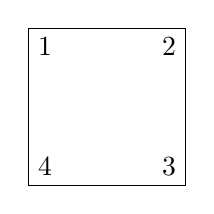
\begin{tikzpicture}[scale=2]
			\draw (0, 0) rectangle (1, 1);
			\draw (0, 0) node[anchor=south west]{4};
			\draw (1, 0) node[anchor=south east]{3};
			\draw (1, 1) node[anchor=north east]{2};
			\draw (0, 1) node[anchor=north west]{1};
		\end{tikzpicture}
	\end{equation*}
	so that the symmetries produce obvious permutations of the set $\left\lbrace 1, 2, 3, 4 \right\rbrace$.
	Namely, the ``pure'' rotations are the following: \begin{equation*}
		\begin{pmatrix*}
			1 & 2 & 3 & 4 \\
			1 & 2 & 3 & 4
		\end{pmatrix*},
		\begin{pmatrix*}
			1 & 2 & 3 & 4 \\
			4 & 1 & 2 & 3
		\end{pmatrix*},
		\begin{pmatrix*}
			1 & 2 & 3 & 4 \\
			3 & 4 & 1 & 2
		\end{pmatrix*},
		\begin{pmatrix*}
			1 & 2 & 3 & 4 \\
			2 & 3 & 4 & 1
		\end{pmatrix*}.
	\end{equation*}
	These correspond to (or ``are mapped to by'') the clockwise rotations $0^\circ$, $90^\circ$, $180^\circ$, and $270^\circ$ respectively.
	If we let $r$ by the $90^\circ$ clockwise rotation, then these correspond to $r^0, r^1, r^2,$ and $r^3$ respectively.
	Also, we can flip along the following lines: northwest to southeast, southwest to northeast, west to east, and finally north to south.
	These correspond to the following permutations (respectively): \begin{equation*}
		\begin{pmatrix*}
			1 & 2 & 3 & 4 \\
			1 & 4 & 3 & 2
		\end{pmatrix*},
		\begin{pmatrix*}
			1 & 2 & 3 & 4 \\
			3 & 2 & 1 & 4
		\end{pmatrix*},
		\begin{pmatrix*}
			1 & 2 & 3 & 4 \\
			4 & 3 & 2 & 1
		\end{pmatrix*},
		\begin{pmatrix*}
			1 & 2 & 3 & 4 \\
			2 & 1 & 4 & 3
		\end{pmatrix*}.
	\end{equation*}
\end{proof}

\begin{ex}
	Describe generators and relations for all dihedral groups $D_{2n}$.
	(Hint: Let $x$ be the reflection about a line through the center of a regular $n$-gon and a vertex, and let $y$ be the counterclockwise rotation by $2\pi / n$. The group $D_{2n}$ will be generated by $x$ and $y$, subject to three relations. To see that these relations really determine $D_{2n}$, use them to show that any product $x^{i_1}y^{i_2}x^{i_3}y^{i_4} \cdots$ equals $x^iy^j$ for some $i, j$ with $0 \leq i \leq 1$, $0 \leq j < n$.)
\end{ex}
\begin{proof}
	Let $e$ be the identity, $x$ the reflection about a line through the center of a regular $n$-gon and one of its vertices, and $y$ the clockwise rotation by $2\pi/n$.
	These are paired with the obvious relations $x^2 = e$ and $y^n = e$, along with the relation $yx = xy^{n - 1}$.

	To prove this, we use induction to show that any product $x^{i_1}y^{i_2}x^{i_3}y^{i_4}\cdots$ for integers $i_1, i_2, i_3, i_4$ equals $x^iy^j$ for some $i, j$ with $0 \leq i \leq 1$ and $0 \leq j < n$.
	It will suffice to show this for all nonnegative integers, since any product including negative exponents can be converted into one including only nonnegative exponents using the relations $x^{-1} = x$ and $y^{-1} = y^{n - 1}$, which derive from the proposed generating relations.
	Given $i_1, i_2 \in \mathbb{Z}^{\geq 0}$ (our base case), \begin{equation*}
		x^{i_1}y^{i_2} = x^{i_1 \bmod 2}y^{i_2 \bmod n}
	\end{equation*}
	since $x^2 = e$ and $y^n = e$.
	Of course, $0 \leq i_1 \bmod 2 \leq 1$  and $0 \leq i_2 \bmod n < n$, so our base case holds.

	We now prove a small lemma: for any $i \in \mathbb{Z}^{\geq 0}$ and $j \in \left\lbrace 0, 1 \right\rbrace$, \begin{equation*}
		y^ix^j = x^jy^k \tag{1}
	\end{equation*}
	for some $k \in \mathbb{Z}^{\geq 0}$.
	First, observe that if $i = 0$ or $j = 0$, (1) is obvious, so we can assume $i > 0$ and $j = 1$.
	We proceed by induction over $i$.
	The case $i = 1$ is already given since $yx = xy^{n - 1}$.
	If $i > 1$ and (1) holds for $i - 1$,
	Then \begin{align*}
		y^ix & = y^{i - 1}yx         \\
		     & = y^{i - 1}xy^{n - 1} \\
		     & = xy^ky^{n - 1}       \\
		     & = xy^{k + n - 1}
	\end{align*}
	for some $k \in \mathbb{Z}^{\geq 0}$.
	Thus (1) holds for all nonnegative integers $i$.

	Now, assume that, for some $m$, $x^{i_1}y^{i_2}\cdots x^{i_{2m - 3}}y^{i_{2m - 2}} = x^iy^j$ for some $i, j$ with $0 \leq i \leq 1$ and $0 \leq j < n$.
	Then for some $j_1, j_2, k_1, k_2, k_3 \in \mathbb{Z}^{\geq 0}$ such that each $0 \leq j_\alpha \leq 1$ and each $0 \leq k_\beta < n$, \begin{align*}
		x^{i_1}y^{i_2}\cdots x^{i_{2m - 1}}y^{i_{2m}} & = x^{j_1}y^{k_1}x^{i_{2m - 1}}y^{i_{2m}} \\
		                                              & = x^{j_1}y^{k_1}x^{j_2}y^{k_2}           \\
		                                              & = x^{j_1}x^{j_2}y^{k_3}y^{k_2}           \\
		                                              & = x^{j_1 + j_2}y^{k_3 + k_2},
	\end{align*}
	leaving us with our already-proven base case.
\end{proof}

\begin{ex}
	For every positive integer $n$ construct a group containing elements $g, h$ such that $|g| = 2$, $|h| = 2$, and $|gh| = n$.
	(Hint: For $n > 1$, $D_{2n}$ will do.)
\end{ex}
\begin{proof}
	For $n = 1$, any group with an element $g$ of order $2$ (e.g. $S_2$) satisfies $|g^2| = |e| = 1$.
	For $n > 1$, consider $D_{2n}$ with generators and relations as described in the previous exercise.
	Then \begin{align*}
		(yx)^2 & = yxyx         \\
		       & = yxxy^{n - 1} \\
		       & = yy^{n-1}     \\
		       & = y^n          \\
		       & = e,
	\end{align*}
	so $|yx| = 2$.
	Thus letting $g = yx$ and $h = x$ satisfies the desired property since $|gh| = |yxx| = |y| = n$.
\end{proof}

\begin{ex}
	Find all elements of $D_{2n}$ that commute with every other element.
	(The parity of $n$ plays a role.)
\end{ex}
\begin{proof}
	If $n$ is odd, then the only element that commutes with every other element seems to be $e$.
	If $n$ is even, however, then we have the case of \begin{align*}
		y^{n / 2}x & = xy^{(n - 1) (n / 2)}                     \\
		           & = xy^{n^2 / 2 - n / 2}                     \\
		           & = xy^{(n^2 / 2 - n / 2) \bmod n}           \\
		           & = xy^{(n^2 / 2) \bmod n - (n / 2) \bmod n} \\
		           & = xy^{- (n / 2) \bmod n}                   \\
		           & = xy^{n / 2},
	\end{align*}
	so $y^{n / 2}$ commutes with $x$, and given any element of $D_{2n}$ expressed as $x^iy^j$ where $0 \leq i \leq 1$ and $0 \leq j < n$ as in Exercise 2.5, we have \begin{align*}
		y^{n / 2}x^iy^j & = x^iy^{n / 2}y^j  \\
		                & = x^iy^{n / 2 + j} \\
		                & = x^iy^{j + n / 2} \\
		                & = x^iy^jy^{n / 2},
	\end{align*}
	so $y^{n/2}$ commutes with every element, as does $e$.
\end{proof}

\begin{ex}
	Find the orders of the groups of symmetries of the five `platonic solids'.
\end{ex}
\begin{proof}
	UNFINISHED
\end{proof}

\begin{ex}
	Verify carefully that `congruence mod $n$' is an equivalence relation.
\end{ex}
\begin{proof}
	Let $\sim$ be the relation ``congruence mod $n$''.
	Given $x, y, z \in \mathbb{Z}$, clearly $n | x - x$, so $\sim$ is reflexive.
	If $x \sim y$, then for some integer $a$, $y - x = an$, so $x - y = -an$, implying that $y \sim x$.
	Finally, if $x \sim y$ and $y \sim z$, let $y - x = an$ and $z - y = bn$ for some integers $a, b$.
	Then $z - x = (z - y) + (y - x) = bn + an = (b + a)n$, so $x \sim z$.
\end{proof}

\begin{ex}
	Prove that $\mathbb{Z}/n \mathbb{Z}$ consists of precisely $n$ elements.
\end{ex}
\begin{proof}
	Clearly $\mathbb{Z}/n \mathbb{Z}$ contains \textit{at least} $n$ elements, since given integers $j, k \in \left\lbrace 0, \dots, n - 1 \right\rbrace$, $n \,|\, k - j$ if and only if $k = j$.
	If $x \in \mathbb{Z}$ and $x \geq n$ or $x < 0$, then there are unique $a, b \in \mathbb{Z}$ such that $0 \leq b < n$ and $x = an + b$, and $a \neq 0$, so $x - b = an$, meaning $n \,|\, x - b$ and $b \equiv x \bmod n$.
	Thus $[b]_n = [x]_n$, so there are no more than $n$ elements of $\mathbb{Z}/n \mathbb{Z}$, and thus $|\mathbb{Z}/n \mathbb{Z}| = n$.
\end{proof}

\begin{ex}
	Prove that the square of every odd integer is congruent to 1 modulo 8.
\end{ex}
\begin{proof}
	We proceed by induction.
	Obviously $1^2 = 1$ is congruent to 1 modulo 8, so let $n$ be some odd integer such that $(n - 2)^2 \equiv 1 \bmod 8$.
	We can write $8a = (n - 2)^2 - 1$ and $n - 1 = 2b$, where $a$ and $b$ are integers.
	Then \begin{align*}
		n^2 - 1 & = ((n - 2) + 2)^2 - 1           \\
		        & = (n - 2)^2  + 4(n - 2) + 4 - 1 \\
		        & = 8a + 1 + 4(n - 1) - 1         \\
		        & = 8a + 4(2b)                    \\
		        & = 8(a + b),
	\end{align*}
	so $n^2 \equiv 1 \bmod 8$.
\end{proof}

\begin{ex}
	Prove that there are no nonzero integers $a, b, c$ such that $a^2 + b^2 = 3c^2$.
	(Hint: By studying the equation $[a]_4^2 + [b]_4^2 = 3[c]_4^2$ in $\mathbb{Z}/4 \mathbb{Z}$, show that $a, b, c$ would all have to be even. Letting $a = 2k, b = 2\ell, c = 2m$, you would have $k^2 + \ell^2 = 3m^2$. What's wrong with that?)
\end{ex}
\begin{proof}
	Note that \begin{align*}
		 & [0]_4^2 = [0]_4  \\
		 & [1]_4^2 = [1]_4  \\
		 & [2]_4^2 = [0]_4  \\
		 & [3]_4^2 = [1]_4.
	\end{align*}
	Let $a, b, c$ be nonzero integers such that $a^2 + b^2 = 3c^2$.
	Then $[a]_4^2$ is either $[0]_4$ or $[1]_4$ since those are the only possible values of squared elements in $\mathbb{Z}/4 \mathbb{Z}$, and likewise for $[b]_4^2$ and $[c]_4^2$.
	Thus $3[c]_4^2$ is either $[0]_4$ or $[3]_4$.
	It cannot be $[3]_4$, however, since any assignment of $[0]_4$ or $[1]_4$ for $[a]_4^2$ and $[b]_4^2$ sums to at most $[2]_4$.
	Thus $3[c]_4^2 = [0]_4$, so $[c]_4^2 = [0]_4$, which forces $[a]_4^2 = [b]_4^2 = [0]_4$ since they must add to $[0]_4$.
	Given this fact, together with the note at the beginning of this proof, $[a]_4$, $[b]_4$, and $[c]_4$ must be either $[0]_4$ or $[2]_4$.
	Therefore, $a$, $b$, and $c$ are all even.

	Let $a = 2k$, $b = 2\ell$, and $c = 2m$.
	Then \begin{align*}
		         & a^2 + b^2 = c^2       \\
		\implies & 4k^2 + 4\ell^2 = 4m^2 \\
		\implies & k^2 + \ell^2 = m^2.
	\end{align*}
	If $k$, $\ell$, and $m$ are all even, there is no issue yet, but we can apply this procedure of dividing $a$, $b$, and $c$ by 2 until an odd number is reached, which would then contradict our finding that all three bases must be even.
\end{proof}

\begin{ex}
	Prove that if $\gcd(m, n) = 1$, then there exist integers $a$ and $b$ such that \begin{equation*}
		am + bn = 1.
	\end{equation*}
	(Use Corollary 2.5.)
	Conversely, prove that if $am + bn = 1$ for some integers $a$ and $b$, then $\gcd(m, n) = 1$.
\end{ex}
\begin{proof}
	By Corollary 2.5, $[m]_n$ generates $\mathbb{Z}/n \mathbb{Z}$, so there exists an integer $a$ such that $a[m]_n = [am]_n = [1]_n$.
	Thus, by definition of $Z/n \mathbb{Z}$, $n\,|\,1 - am$, so there exists an integer $b$ such that $bn = 1 - am$.

	Conversely, if $am + bn = 1$ for integers $a$ and $b$, then $bn = 1 - am$, so $n\,|\,1 - am$, meaning $[1]_n = [am]_n = a[m]_n$ in $\mathbb{Z}/n \mathbb{Z}$.
	Thus given any $[\ell]_n \in \mathbb{Z}/n \mathbb{Z}$, $[\ell]_n = \ell[1]_n = \ell a [m]_n$, so $[m]_n$ generates $\mathbb{Z}/n \mathbb{Z}$.
	By Corollary 2.5, then, $\gcd(m, n) = 1$.
\end{proof}

\begin{ex}
	State and prove an analog of Lemma 2.2, showing that the multiplication on $\mathbb{Z}/n \mathbb{Z}$ is a well-defined operation.
\end{ex}
\begin{proof}
	We need to show that if $a \equiv a'\bmod n$ and $b \equiv b' \bmod n$, then \begin{equation*}
		ab \equiv a'b' \bmod n.
	\end{equation*}

	Let $a \equiv a' \bmod n$ and $b \equiv b' \bmod n$.
	Then $xn = a' - a$ and $yn = b' - b$ for some integers $x$ and $y$.
	Thus \begin{align*}
		a'b' - ab & = (xn + a)(yn + b) - ab       \\
		          & = xyn^2 + ayn + bxn + ab - ab \\
		          & = n(xyn + ay + bx),
	\end{align*}
	so $ab \equiv a'b' \bmod n$ as desired.
\end{proof}

\begin{ex}
	Let $n > 0$ be an odd integer.
	\begin{itemize}
		\item Prove that if $\gcd(m, n) = 1$, then $\gcd(2m + n, 2n) = 1$.
		      (Use Exercise 2.13.)
		\item Prove that if $\gcd(r, 2n) = 1$, then $\gcd(\frac{r + n}{2}, n) = 1$. (Ditto.)
		\item Conclude that the function $[m]_n \to [2m + n]_{2n}$ is a bijection between $(\mathbb{Z}/n \mathbb{Z})^*$ and $(\mathbb{Z}/2n \mathbb{Z})^*$.
	\end{itemize}
	The number $\phi(n)$ of elements of $(\mathbb{Z}/n \mathbb{Z})^*$ is \textit{Euler's $\phi$-function}.
	The reader has just proved that if $n$ is odd, then $\phi(2n) = \phi(n)$.
	Much more general formulas will be given later on.
\end{ex}
\begin{proof}\
	\begin{itemize}
		\item Since $n$ is odd and $\gcd(m, n) = 1$, $\gcd(2m, n) = 1$ as well because no factor of $n$ divides $m$ and 2 is not a factor of $n$.
		      Therefore, $[2m]_n = [2m + n]_n$ generates $\mathbb{Z}/n \mathbb{Z}$, so $\gcd(2m + n, n) = 1$.
		      Finally, since $2m$ is even and $n$ is odd, $2m + n$ is odd, so by the same logic we started with, $\gcd(2m + n, 2n) = 1$.
		\item Since $\gcd(r, 2n) = 1$, $r$ must be odd, so $\gcd(r, n) = 1$.
		      This means that $[r]_n = [r + n]_n$ generates $\mathbb{Z}/n \mathbb{Z}$, so in fact $\gcd(r + n, n) = 1$.
		      Finally, since both $r$ and $n$ are odd, $r + n$ must be even, so $\frac{r + n}{2}$ is an integer and we get $\gcd(\frac{r + n}{2}, n) = 1$.
		\item Let $[m]_n \in (\mathbb{Z}/n \mathbb{Z})^*$.
		      Then, by definition, $\gcd(m, n) = 1$, and we can define $f: (\mathbb{Z}/n \mathbb{Z})^* \to (\mathbb{Z}/{2n}\mathbb{Z})^*$ by $f([m]_n) = [2m + n]_{2n}$.
		      First we show that this is well defined by letting $[m_1]_n = [m_2]_n$, so that $m_2 - m_1 = an$ for some integer $a$, and thus \begin{equation*}
			      (2m_2 + n) - (2m_1 + n) = 2(m_2 - m_1) = 2an,
		      \end{equation*}
		      which is divisible by $2n$ as desired.

		      Now assume that $f([m_1]_n) = f([m_2]_n)$ for some $m_1, m_2$ relatively prime to $n$.
		      Then by definition there exists some integer $a$ such that \begin{equation*}
			      an = (2m_2 + n) - (2m_1 + n) = 2(m_2 - m_1).
		      \end{equation*}
		      Thus $n$ divides $m_2 - m_1$ (it cannot divide 2), so $[m_1]_n = [m_2]_n$ and $f$ is injective.

		      Given $[m]_{2n} \in (\mathbb{Z}/{2n}\mathbb{Z})^*$, we know that $\gcd(m, 2n) = 1$, so by the second bullet point, $\gcd(\frac{m + n}{2}, n) = 1$.
		      This helps because, in fact, \begin{align*}
			      f\left(\left[\frac{m + n}{2}\right]_n\right) & = \left[ 2\left(\frac{m + n}{2}\right) + n \right]_{2n} \\
			                                                   & = \left[ m + 2n \right]_{2n}                            \\
			                                                   & = \left[ m \right]_{2n}.
		      \end{align*}
		      Thus $f$ is bijective.
	\end{itemize}
\end{proof}

\begin{ex}
	Find the last digit of $1238237^{18238456}$.
	(Work in $\mathbb{Z}/10 \mathbb{Z}$.)
\end{ex}
\begin{proof}
	Exercise 2.14 implies that exponentiation is well-defined on $\mathbb{Z}/n \mathbb{Z}$ since \begin{equation*}
		[a^b]_n = [\underbrace{a \cdots a}_{\text{$b$ times}}]_n = \underbrace{[a]_n \cdots [a]_n}_{\text{$b$ times}} = [a]_n^b.
	\end{equation*}
	Furthermore, \begin{equation*}
		[a]_n^b = [a]_n^{(b \bmod |[a]_n|)}.
	\end{equation*}
	In the present case, of course $[1238237]_{10} = [7]_{10}$, and the order of $[7]_{10}$ is 4, as is easily checked.
	This allows us to conclude that \begin{align*}
		[1238237^{18238456}]_{10} & = [1238237]_{10}^{18238456}   \\
		                          & = [7]_{10}^{18238456}         \\
		                          & = [7]_{10}^{18238456 \bmod 4} \\
		                          & = [7]_{10}^{0}                \\
		                          & = [1]_{10}.
	\end{align*}
	Thus the last digit of $1238237^{18238456}$ is 1.
\end{proof}

\begin{ex}
	Show that if $m \equiv m' \bmod n$, then $\gcd(m, n) = 1$ if and only if $\gcd(m', n) = 1$.
\end{ex}
\begin{proof}
	($\implies$) Given $\gcd(m, n) = 1$, since $m \equiv m' \bmod n$ we have $an = m' - m$ for some integer $a$.
	Then we simply have \begin{align*}
		[m]_n & = [m + an]_n     \\
		      & = [m + m' - m]_n \\
		      & = [m']_n.
	\end{align*}

	($\impliedby$) The opposite direction follows by the same logic, interchanging the roles of $m'$ and $m$.
\end{proof}

\begin{ex}
	For $d \leq n$, define an injective function $\mathbb{Z}/d \mathbb{Z} \to S_n$ preserving the operation, that is, such that the sum of equivalence classes in $\mathbb{Z}/d \mathbb{Z}$ corresponds to the product of the corresponding permutations.
\end{ex}
\begin{proof}
  UNFINISHED
\end{proof}

\begin{ex}
	Both $(\mathbb{Z}/5 \mathbb{Z})^*$ and $(\mathbb{Z}/12 \mathbb{Z})^*$ consist of 4 elements.
	Write their multiplication tables, and prove that no re-ordering of the elements will make them match.
\end{ex}
\begin{proof}
	It is easy to see that \begin{equation*}
		(\mathbb{Z}/5 \mathbb{Z})^* = \left\lbrace [1]_5, [2]_5, [3]_5, [4]_5 \right\rbrace
	\end{equation*}
	and \begin{equation*}
		(\mathbb{Z}/12 \mathbb{Z})^* = \left\lbrace [1]_5, [5]_5, [7]_5, [11]_5 \right\rbrace.
	\end{equation*}
	For the former, we have the multiplication table (omitting the brackets and subscripts when denoting $[*]_5$) \begin{equation*}
		\begin{tabular}{ c || c | c | c | c }
			  & 1 & 2 & 3 & 4 \\ \hline \hline
			1 & 1 & 2 & 3 & 4 \\ \hline
			2 & 2 & 4 & 1 & 3 \\ \hline
			3 & 3 & 1 & 4 & 2 \\ \hline
			4 & 4 & 3 & 2 & 1 \\
		\end{tabular}
	\end{equation*}
	and for the later we have \begin{equation*}
		\begin{tabular}{ c || c | c | c | c }
			   & 1  & 5  & 7  & 11 \\ \hline \hline
			1  & 1  & 5  & 7  & 11 \\ \hline
			5  & 5  & 1  & 11 & 7  \\ \hline
			7  & 7  & 11 & 1  & 5  \\ \hline
			11 & 11 & 7  & 5  & 1  \\
		\end{tabular}
	\end{equation*}

  From this we can see that $\mathbb{Z}/5 \mathbb{Z}$ has exactly one element of order 2, and in $\mathbb{Z}/12 \mathbb{Z}$ three elements have order 2, so they cannot be the same.
\end{proof}

\end{document}
